%\documentclass[a4paper, twocolumn]{article}
\documentclass[a4paper]{article}
\newcommand{\papertitle}{Potential of I/O-Aware Workflows in Climate and Weather}

\usepackage[a4paper, margin=2cm]{geometry}

\usepackage[utf8]{inputenc}
\usepackage[T1]{fontenc}
\usepackage{graphicx}
\usepackage[english]{babel}
\usepackage[colorlinks=true,urlcolor=red]{hyperref}
\usepackage{url}
\usepackage{float}
\usepackage{cleveref}
\usepackage{todonotes}
\usepackage{comment}
\usepackage{ulem}
\usepackage{array}
\usepackage{subcaption}

\newcommand{\jk}[1]{\todo[inline]{JK: #1}}
\newcommand{\lr}[1]{\textcolor{blue}{LR: #1}}

\usepackage{multicol}
\setlength{\columnsep}{1cm}

\usepackage{fancyhdr}
\fancyhead{}
\fancyfoot{}
\fancyhead[l]{\papertitle}
\fancyhead[r]{
\includegraphics[height=1em]{esiwacelogo_type_grey_left_2c_ext}}
\fancyfoot[r]{\thepage}
\pagestyle{fancy}
\renewcommand{\headrulewidth}{1pt}
\renewcommand{\footrulewidth}{1pt}

\usepackage{titling}
\pretitle{\begin{center}\Large\bfseries}
\posttitle{\end{center}\vskip 0.5em}

\graphicspath{{./assets/}}

\title{\papertitle}

\author{
%  Julian M. Kunkel
%  \textit{University of Reading}
%    \and
%  Luciana R. Pedro
%  \textit{University of Reading}
}
\date{\today}


\begin{document}
\maketitle
\thispagestyle{fancy}

\section*{Abstract}
The efficient, convenient, and robust execution of data-driven workflows and enhanced data management are key for productivity in scientific computing.
Traditionally, in HPC, the concerns of storage and computing are separated and optimised independently from each other and the needs of the end-to-end user.
As climate and weather workflows become increasingly complex and blend beyond data centres while, at the same time, storage hierarchies become deeper, the community investigates means to re-organise storage access to utilise such environments fully.

The key contributions of this paper are:
1) we sketch the visions of an integrated data-driven approach and discuss the challenges and implications of this strategy;
2) we illustrate architecture and roadmap that allows the seamless integration into existing workflows.
The tools employed here to achieve this extended workflow are Cylc, XIOS, DDN IME, and ESDM.

%Basically, we believe workflows composed of data, computing, and communication-intensive tasks should drive the interfaces and hardware configurations to best support the programming models.
From the user perspective, we ultimately aim to provide an abstraction to data dependencies.
The proposed changes increase the opportunity of implementations for smarter scheduling of computing and storage in heterogeneous storage environments considering characteristics of workflows and data.
From the system perspective, the vision aims to derive an execution plan that utilises the available hardware and software infrastructure within a data centre.


\section{Introduction}

High-Performance Computing (HPC) harnesses the fastest hardware components to enable the execution of tightly coupled applications from science and industry.
Typical use-cases cover the numerical simulation of physical systems and the analysis of large-scale observational data.
In the domain of climate and weather, there is a considerable demand for the orchestration of ensembles of simulation models and the generation of data products.
A weather forecast service such as ECMWF generates .... \jk{Cylc team, please provide some facts}
Likewise, ensembles in climate can ...

Based on their needs, the HPC community has developed a software ecosystem that supports them to execute their large-scale workflows.
While the current advances correspond to a big leap forward, many processes still require experts.
For example, porting a workflow from one system to another requires to adjust runtime parameters of applications and to decide how data is managed.
Since performance is of crucial importance to large-scale workflows, careful attention must be paid to exploit the system characteristics of the target supercomputer.
To obtain the best performance, a specific supercomputer typically requires substantial changes to the workflow to tailor the workflow to the particular machine.
For instance, a data-driven workflow may benefit from using a heterogeneous set of computing and storage technology at the same time.

Knowing the capabilities, interfaces, and performance characteristics of individual components are mandatory to make the best use of them.
As the complexity of systems increases and alternative storage and computing technologies provide unique characteristics, it becomes increasingly difficult even for experts to manually optimise resource usage in workflows. In many cases, modifications are not performed because: 1) they are labour intense: any change to the workflow requires careful validation which may not pay off for small scale runs; 2) users are not aware of the potential of the complex system.

In this paper, we show that knowledge about Input/Output of workflow tasks and overall experimental design helps to
optimise the execution of climate and weather workflows and may increase the performance, throughput and cost-efficiency of the environments, providing an incentive to users and data-centres that cannot be neglected.

%The paper is organised as follows:
%In \Cref{sec:workflows}, we provide an overview of the specification of workflows in climate and weather and the involved software stack.

\jk{TODO}


\section{Workflows in Climate/Weather}
\label{sec:workflows}

In this section, we describe how the environment workflows are executed in the typical software stack.

\subsection{Data Center Infrastructure}

To satisfy the needs for different workflows, data centres are providing a infrastructure consisting of computing and storage devices with different characteristics which makes them more efficient for specific tasks.
Take, for example, the supercomputer Mistral at DKRZ that consists of 3,321 nodes.
It offers two types of compute nodes equipped with different CPUs and a range of GPU nodes.
Each node provides an SSD for local storage, and DKRZ has additionally two shared Lustre file systems with different performance characteristics.
Individual users and projects are mapped to one file system explicitly, and users can access it as work or scratch file system: While data is kept on the work file system indefinitely, its available space is limited by a quota.
The scratch file system allows to store more data, but data is automatically deleted after some time.

Future centres are expected to have even more heterogeneity. A variety of accelerators (GPU, TPU, FPGAs), active storage, in-memory, and in-network computing technologies provide storage and processing capabilities.
\Cref{fig:heterogeneous} shows such an environment with a focus on computation and storage.
Some of these technologies might be local to specific compute nodes or globally available.
Depending on the need, the storage characteristics range from predictable low-latency (in-memory storage, NVMe) to online storage (SSD, HDD), and cheap storage for long-term archival (tape).
\jk{Mention BBs, e.g., DDN IME}
Naturally, the variety of tasks executed by a single workflow may benefit from the different storage and computing infrastructure.

\begin{figure}[H]
  \centering
  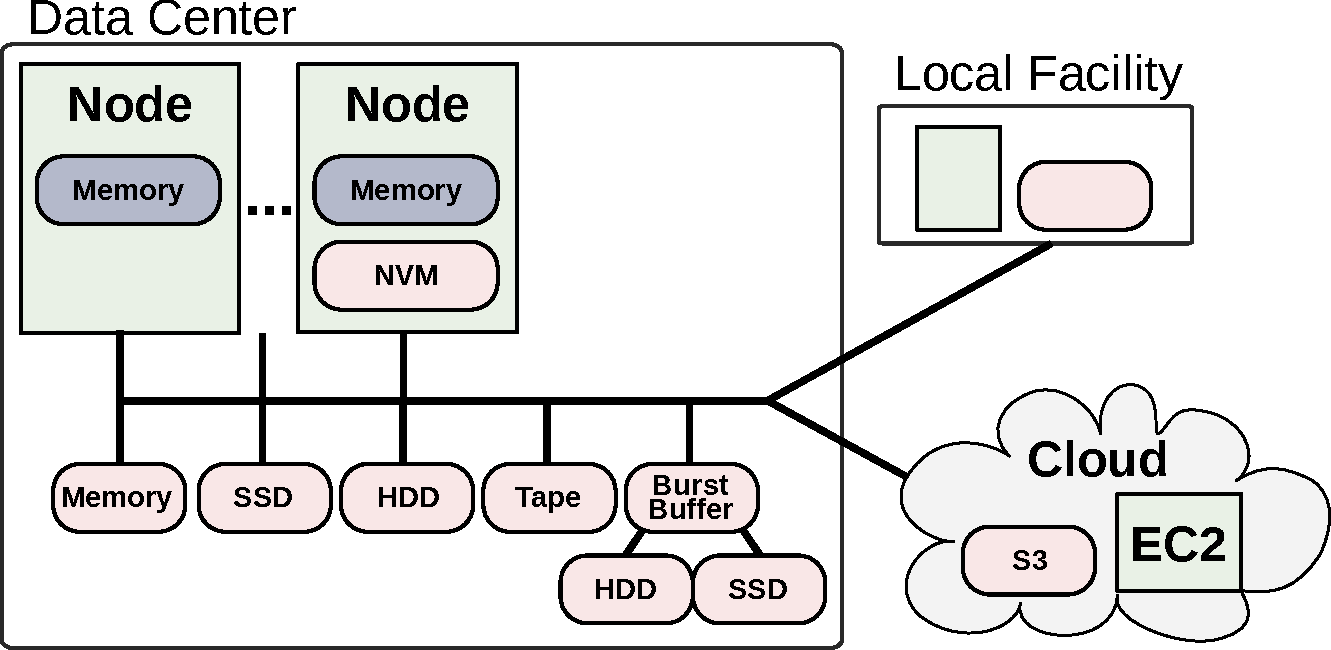
\includegraphics[width=0.6\columnwidth]{system}
  \caption{Example of an heterogeneous HPC landscape}
  \label{fig:heterogeneous}
\end{figure}


\subsection{I/O Stack of a Parallel Application}

A typical I/O stack for a single parallel application like a climate model is shown in \Cref{fig:layers}.

\begin{minipage}{0.2\textwidth}
\begin{figure}[H]
  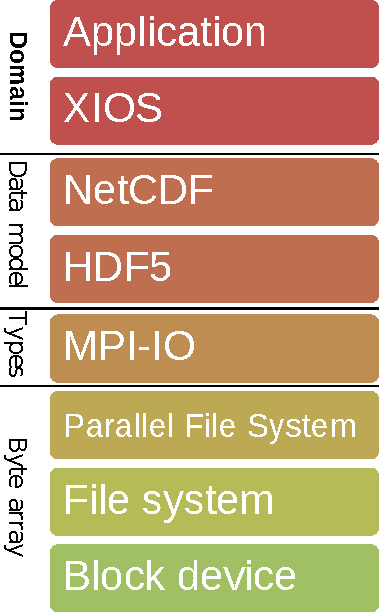
\includegraphics[width=\textwidth]{layers-xios}
  \caption{I/O path for an MPI-parallel application}
  \label{fig:layers}
\end{figure}
\end{minipage}
\qquad
\begin{minipage}{0.7\textwidth}
In our example, we assume the application is parallelised for performance reasons and uses MPI to run the application.
It may use XIOS to gather data from individual fields which then uses NetCDF4 to store the data as a file.
XIOS provides a domain-level semantics and ...\jk{TODO}
Under the hood, NetCDF4 used the HDF5 API and file format.
Internally, HDF5 uses MPI again and its data types to specify the nature of the data stored.
Finally, data is stored on a parallel file system like Lustre, which, on the server-side, stores data in the local file system as block devices on storage media such as SSDs and HDDs.

Different applications involved in a workflow may use a different I/O stack to store their outputs.
Naturally, the application that inputs previously generated data must use a compatible API to be able to read the specific data format.
In this figure, for example, XIOS is beneficial for parallel I/O and a process might directly rely on the NetCDF API to read previous data.

Within ESiWACE, we are developing ESDM, ... \jk{TODO}
\end{minipage}



\subsection{Software Stack}

The appropriate software stack involved in executing a workflow is depicted in \Cref{fig:stages}.
As a preliminary, the user had specified a Cylc suite representing the workflow and provided scripts files for the individual tasks to execute; now the user enacts Cylc to start the workflow.
In the following, each stage of the execution is described further.

\begin{figure}[H]
  \centering
  
\includegraphics[scale=1.4]{stages}
  \caption{Software stack and stages of execution}
  \label{fig:stages}
\end{figure}



\begin{enumerate}
  \item \textbf{Cylc} Cylc parses the suite file, generate dependencies and defines a schedule for the execution.
  Cylc monitors the progress of the workflow.
  Once a task can be executed (dependencies are fulfilled), Cylc generates a Slurm script on the fly with the required metadata for Slurm that will invoke the user-defined script for that task and runs Slurm to queue the job.

  \item \textbf{Slurm} Slurm schedules the execution of the job considering the scheduling policy of the data centre.
  Once the job is ready to be dispatched, i.e., resources are available, and the job priority is the highest, it is started on the supercomputer.

  \item \textbf{Job} The user-provided script is executed on a single node assigned to the job.
  The script has set environment variables containing information about the Cylc execution (e.g., a task in the workflow) and the Slurm job (e.g., number of nodes).

  \item \textbf{Script} The shell-script executes the sequence of commands, including applications that are parallel programs.
  Typically, to create a filename, the script calls Cylc commands with a template provided by the user and feeds this information to the application which, ultimately, defines the storage location to be used.
  A script typically consists of multiple fine-grained commands and may even call multiple parallel applications.

  \item \textbf{Application} The user-specified parallel application runs taking the filenames as defined in a configuration file or as arguments.
  The application may use NetCDF or XIOS to perform the I/O.
\end{enumerate}


\subsection{Cylc}

Cylc is in charge to execute and monitor workflows in which each step is submitted to the batch scheduler of a data centre.
 %, and the relevance of heterogeneous infrastructure to run workflows.
%We focus on high-level considerations to illustrate mandatory concepts.



Consider the Cylc suite configuration for a toy monthly cycling workflow in \Cref{fig:cylc} \cite{8675433}.
In this workflow, a warm-cycled atmospheric model (\textbf{model}) simulates the physics from a current state to predict the future after a timestep, for example, after six hours.
This process is repeated in the model to simulate month and years into the future.
Once the simulation of any month is computed, the data for this month becomes available and can be analysed.
A user has specified a detailed workflow in a Cylc suite file (\texttt{suite.rc}).
In this workflow, the \textbf{model} is followed by postprocessing (\textbf{post}), forecast verification (\textbf{ver}), and product generation (\textbf{prod}) tasks.
Also, consider, in addition, a task \textbf{check} that compares some verification metric against products from two cycles earlier.

\begin{figure}[H]
  \centering
  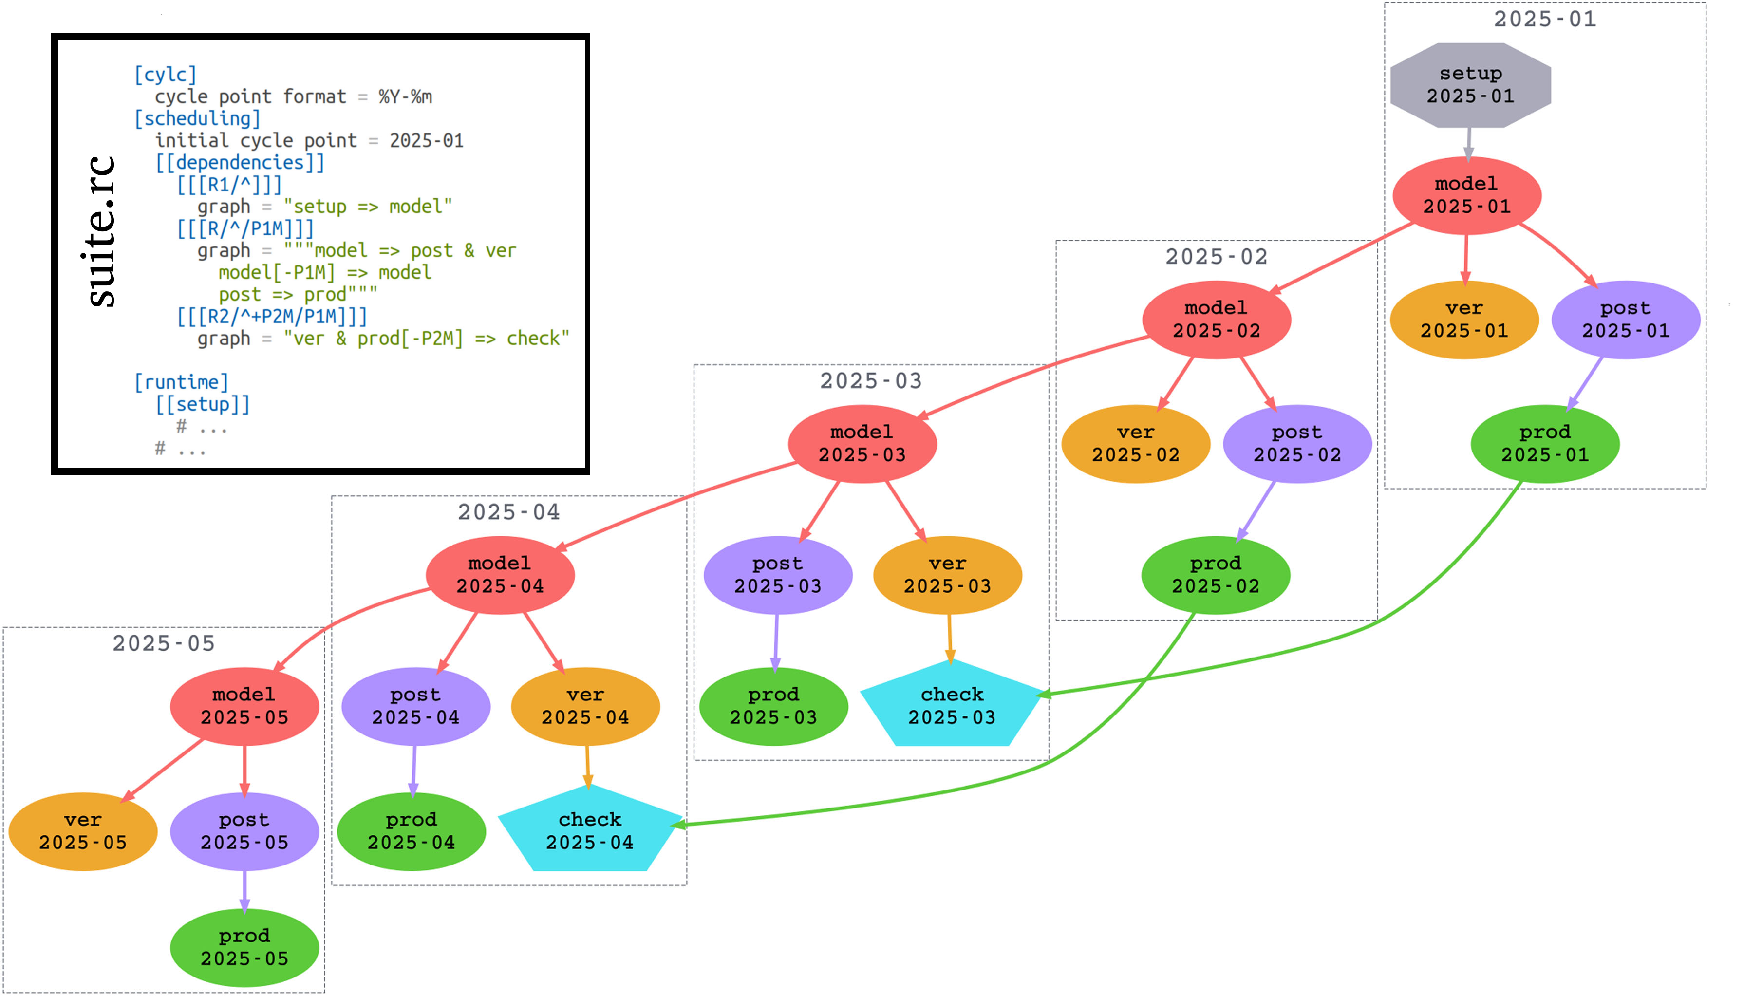
\includegraphics[width=0.9\columnwidth]{cylc1}
  \caption{Example workflow}
  \label{fig:cylc}
\end{figure}

This suite presents the dependencies among the tasks, but it is missing the information about I/O and storage.
Decisions about storage must take into consideration the architecture in which the workflow will run.
The developers make the configuration about parallelism and where the data is stored in a script file that is executed for each specific task.

\subsection{Data Management}
\label{sec:datamanagement}

The scripts for the tasks in Cylc define how the data is stored on the available storage systems.
Consider that the machine has three file systems: a fast \textbf{scratch} file system on which data may reside only for a week, a slower \textbf{work} file system, and each node has a \textbf{local} file system.

What happens in many current workflows is that they use the only \textbf{work} and \textbf{scratch}.
When a task is set to computing, the corresponding dataset is moved to \textbf{scratch}, processed, and the resulting datasets are transferred back to \textbf{work}.
If the \textbf{scratch} filesystem achieves its capacity, then the datasets move back to \textbf{work} and keep running the task until it is finished.
If the I/O planning is made a priori, this situation can be avoided.
In addition to the file systems described, many supercomputers also have available for the user \textbf{scratch2} file systems (sometimes local and global).
Therefore, in a real scenario, if the architecture of the machine is known, we can better utilise its resources.

\Cref{fig:lifecycle} shows three possible life cycles and the access pattern for a specific dataset.
As shown in \Cref{fig:lifecycle1}, the dataset could be stored on the \textbf{local} storage first to avoid congestion on the \textbf{work} file system, then be migrated to \textbf{work} file system where subsequent tasks of the workflow may read it multiple times.
In the end, this dataset might be an intermediate product that can then be deleted.
Alternatively (\Cref{fig:lifecycle2}, it could be stored on the \textbf{scratch} file system immediately and accessed there.
However, that would require that the last read access happens before files on \textbf{scratch} are automatically removed.
The last scenario (\Cref{fig:lifecycle3}) presents the case where data is created on \textbf{work} by a task. Still, then it is copied to a \textbf{local} node to allow read accesses of subsequent tasks which might be beneficial for small random accesses.
However, it would require that the subsequent tasks are placed on the same machine where data is now stored.
The scientist responsible for the workflow must optimise the available resources intuitively.
These are just examples, and currently, the scientists perform such kind of optimisations manually.

\begin{figure}[H]
  \centering
  \begin{subfigure}{.3\textwidth}
  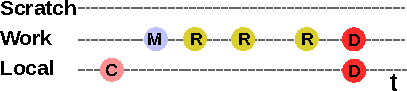
\includegraphics[width=0.9\columnwidth]{lifecycle-1}
  \caption{\label{fig:lifecycle1} Local and work file systems}
  \end{subfigure}
  \begin{subfigure}{.3\textwidth}
  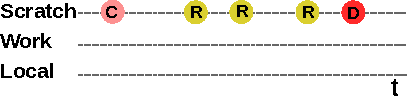
\includegraphics[width=0.9\columnwidth]{lifecycle-2}
  \caption{\label{fig:lifecycle2} Scratch file system only}
  \end{subfigure}
  \begin{subfigure}{.3\textwidth}
  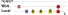
\includegraphics[width=0.9\columnwidth]{lifecycle-3}
  \caption{\label{fig:lifecycle3} Local and work file systems}
  \end{subfigure}
  \caption{Alternative life cycles for mapping a dataset to storage and the operations: \textbf{C}reate, \textbf{M}igrate, \textbf{R}ead, and \textbf{D}elete}
  \label{fig:lifecycle}
\end{figure}


\section{State of the Art}

Manual tiering requires the user or application to control the data placement, i.e., storing data (typically in the form of files on a particular storage system and, usually, moving data between storage by using scripts.
One limitation here is that decisions about how data structures are mapped and packaged into files are made once by the producing application, and cannot be changed without manual intervention by a downstream application.

A policy system (e.g., deployed on a burst buffer) aims to simplify the data movement for the user, but typically migrates objects in the coarse granularity of files.
However, the semantical information that can be used by a policy system to make decisions is limited, e.g., data location, file extension, age of the file, etc.

Other tools for workflow handling, how is this information transported?

dataspaces + ADIOS + in-situ

\jk{TODO}

\cite{Vladimirov2014FileIO}


\section{Vision for I/O-Aware Workflows}

Applied scientists should not spend time understanding hardware characteristics, but using their time to develop their work, let the computer do the job the most straightforward way as possible, and just collect and analyse the results.
However, nowadays, to be able to run a job in a HPC environment efficiently, researchers have to have profound knowledge about their workflow, which is expected, but also about decisions regarding storage, communication, and computing.

Data system do not respect the importance of data depends at all. Aspects like costs to reproduce the data (can it be reproduced easily), the type of the experiment (test run, production run) and runtime constraints for the overall and potential crucial workflow are not considered.
Value and priority should influence fault-tolerance strategies and imply the quality of service for performance and availability.

We propose an approach to reduce the burden on researchers and, at the same time, optimise the decisions about jobs running in HPC systems.
Once we have an automated decision about where the job will run and how the storage will be managed, scientists can then run their workflows in any machine without further interactions and even without previous knowledge about the machine architecture.

Our vision requires two additional information: firstly, the user must augment the workflow description with information about I/O requirements and explicitly annotate dependencies to data sets; secondly, the data centre (or expert user) must provide a description of the storage architecture and characteristics for each storage system.

There are many approaches to implement the technology for this vision. It is apparent that changes need to be made to several software components to realise this vision.
In the next section, we will discuss the specific design for our transitional roadmap for climate and weather.


\subsection{Extended Workflow Description}

So far, Cylc allowed specifying tasks and the dependencies among them.
We aim to enrich this information with characteristics for input, and output, i.e., the datasets used.
An example workflow containing input data sets and (intermediate) products is illustrated in \Cref{fig:workflow}.
Nodes represent tasks or data; arrows indicate dependencies among between them.
In the example, Task\,1 needs two datasets to perform its work, it directly communicates with Task\,2 and produces Product\,1.
Most of the workflow can run automatically, except for the manual quality control of the products and the final data usage of Product\,3.
This last step represents the typical uncertainty of data reuse, i.e., it is unclear how Product\,3 will be used further.
In this approach, each task is annotated with the required inputs and the generated products.
Each data product is annotated with metadata such as data life cycle information, e.g., the value of data and how long should it be kept.

%It was correctly placed here

By monitoring I/O accesses, we can automatically draft such I/O descriptions on behalf of the user to simplify the specification.
All we need is to run one cycle of the specific workflow, considering that a workflow cycle is executed many times in climate and weather; this is a cheap approach.
From the recorded I/O accesses, we analyse the I/O patterns and dependencies associated with it to generate the configuration file.

\begin{figure}[H]
  \centering
  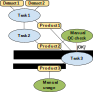
\includegraphics[width=0.4\columnwidth]{workflow}
  \caption{Example of a high-level workflow with tasks and data dependencies}
  \label{fig:workflow}
\end{figure}

\subsection{System Information}

The system information shall comprise of all available storage systems, the system topology, and the characteristics of each of its required components.
This may include simplified or complex models of the components to approximate performance for specific I/O patterns allowing to predict performance behaviour.
It is expected that the data centre (or expert users) can create such a configuration file, for instance, by using vendor-provided information or by executing benchmarks.

\subsection{Smarter I/O Scheduling}

With this separation of concerns, we can abstract from the workflow what is essential and what a machine should optimise to ensure that the resources available are being used smartly.
In this paper, we focus on utilising a heterogeneous storage environment instead of exhaustively discussing the potential that is unleashed with the right level of abstraction in place by researchers that exploit the available opportunities.
Every time parameters are manually tuned right now there is a room from improvement by using automatised decision making.
And Machine Learning has been proven effective in replacing human-beings and adapt the workflow dynamically in case of unexpected situations (the system is down, nodes are unresponsive, etc.).

Optimisations we discuss in this paper are related to the life cycle of datasets and the placement of such datasets into specific storage according to system performance characteristics and the workflow specification.
Firstly, the I/O scheduler could make the placement decision for the individual data sets and manage their relocation during the life cycle, as discussed in \Cref{sec:datamanagement}.

Consider the hypothetical case to have just two tasks A and B that need to be repeated many times:
Datasets generated by Task\,\textbf{A} are used by Task\,\textbf{B} and hence both tasks must have access to the same data in the system.
Because there is one script responsible for setting the configuration, the decision in which directory to store data is somewhat fixed.
Such configuration was done manually and with restricted information about the storage and system architecture.
It would be interesting to explore storage options for the datasets and, e.g., have different cycles stored placed in different storage systems.
If the lifetime of such dataset is, for instance, two cycles, alternate the datasets into two scratch file systems is something that would be a simple job an I/O-aware scheduler.
However, manually, that implies at having at least two scripts\footnote{Complicated scripts would have allowed changing the storage type depending on the cycle. Still, it is a significant burden to the user.} for each task with information about the different storage.

\Cref{fig:cycle4} exemplifies a restriction of our example climate/weather workflow the way it was being generated.
Assume you have, for instance, four cycles of the model running with all the necessary post-processing steps.
Typically, the user has written the scripts for each task by defining a filename using the same prefix that is then placed at the same storage type every time.
That happens because all datasets generated by Task \textbf{model} will be used by Task \textbf{post\,prod}, so they should stay on the same node.
The user-specific storage locations are a viable option to run a workflow.
The user might even have analysed various scenarios such as depicted in
\Cref{sec:datamanagement}.


Additionally, by knowing how to rerun the workflow behind the data creation, a smarter storage system could trade data security with potential recomputation opportunities to optimise the cost-efficiency of the system.
Intermediate states could be rerun by utilising virtualisation and container technologies.
Similarly, the scheduler may decide to couple subsequent steps of a workflow directly without storing intermediate data products on persistent storage.
Finally, data might be replicated but enables the system to rerun parts of the workflow in case of a data loss.

Ultimately, by abstracting and automatizing these tasks, we provide a smarter route taking into consideration the architecture available and the way the datasets are stored during the intermediate steps of the workflow.


\begin{figure}[H]
  \centering
  \includegraphics[width=0.8\columnwidth]{cycle4}
  \caption{Four stages workflow example}
  \label{fig:cycle4}
\end{figure}


\subsection{Benefit}

Once we have the complete knowledge about how the workflow is expected to run, we can optimise steps that were before predefined by the user, usually considering only options for feasibility.

\begin{itemize}
\item Abstraction: The user does not have to worry about the architecture that the workflow will run, removing the specialist from the decision-making process.

\item Optimisation: The workflow will be optimised for the specific available system characteristics considering potentially runtime characteristics and storage resilience which will increase performance and system utilisation.
By knowing the workflow behind the data creation, the system could trade data security with potential recomputation opportunities to optimise the cost-efficiency.

\item Performance-portability: The user has to specify the I/O requirements only once for the tasks of the workflow.
The workflow can now be run on any system without user intervention.
Even more, if the system characteristics change, e.g., it gets upgraded, and an additional storage tier becomes available, or if storage degrades, the I/O-aware workflow could automatically adapt and make use of this new environment.

\end{itemize}


\section{Design}

This section describes our approach to incrementally extend the current software stack for climate and weather workflows which realises parts of our vision.
To automatically make scheduling decisions, the software stack needs to:

\begin{enumerate}

\item Delivers information about storage life cycle together with the workflow, and

\item Adapts the resulting workflow, individual scripts and application executions to consider the automatic I/O schedule.

\end{enumerate}

\subsection{Agregatting Data Dependencies}

\Cref{fig:cycle1} introduces one cycle of the suite in \Cref{fig:cylc} with a simplified notation. The arrows represent the tasks dependencies, but there is no information about the data that are generated. Tasks \textbf{verification} and \textbf{post\,proc} depend on Task \textbf{model}, but does Task \textbf{model} needs to be fully completed to satisfy the dependencies?
Of course, once Task \textbf{model} is completed, the dependent tasks can be executed, and that is the type of information Cylc has to create to reproduce the workflow.

\begin{comment}

\begin{figure}[H]
\centering
\begin{tabular}{ccc}
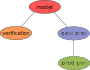
\includegraphics[scale=0.6]{cycle1} & \qquad &
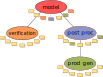
\includegraphics[scale=0.6]{cycle-io-dep} \\
(a) Original Cycle & & (b) Cycle including datasets and dependencies
\end{tabular}
\caption{ \label{fig:cycle} Simplified Cylc workflow for the first cycle}
\end{figure}

\end{comment}

\begin{figure}[H]
  \begin{subfigure}{0.45\textwidth}
    \centering
    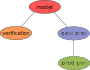
\includegraphics[width=\columnwidth]{cycle1}
    \caption{Original Cycle}
    \label{fig:cycle1}
  \end{subfigure}
  \qquad
  \begin{subfigure}{0.45\textwidth}
    \centering
    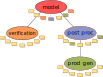
\includegraphics[width=\columnwidth]{cycle-io-dep}
    \caption{Cycle including datasets and dependencies}
    \label{fig:cycle-io-dep}
  \end{subfigure}
  \caption{Simplified Cylc workflow for the first cycle}
\end{figure}

The scenario presented in \Cref{fig:cycle1} shows the same cycle of \Cref{fig:cycle-io-dep}, but  extended information about datasets is added.
In this picture, we have the tasks dependencies, and we explicitly list the datasets dependencies regarding the tasks that generated them.
The way data moves through tasks is by creating datasets to pass on the information, including filename and storage destination.
The datasets produced by every task are coded in the workflow scripts before Cylc evaluation, and it is just replicated by this tool. The tasks can create a different number of datasets, and these datasets may be necessary for the immediate next task in the current cycle, or tasks in different cycles.

Datasets colours indicate which task will use their information and datasets in yellow represent information that will be used in a different cycle. The tricky part when we consider only tasks and not the datasets in the workflow is that it may lead to the false impression that one task depends only on the immediately previous one. Note, for instance, that one dataset produced by Task \textbf{model} is later used in Task \textbf{prod\,gen}. That is not an immediate conclusion when we analyse just the arrows for the dependencies. It is clear that Task \textbf{model} is a dependency for Task \textbf{post\,prod}, which is then a dependency for Task \textbf{prod\,gen}. Still, the crucial information here is that any dataset currently being used in the current cycle can also be used later. From the diagram we can also notice that Task \textbf{model} will generate one dataset for Task \textbf{post\,proc}, one dataset for Task \textbf{prod\,gen}, two datasets for Task \textbf{verification}, and three datasets for later cycles.

The access to this information before the process starts can be used to optimise where compute jobs are executed and how these datasets will be stored during the workflow.
This information today is static and manual, leaving opportunities for automatisation and optimisations open.
The idea here is to embrace the concept that tasks dependencies are really imposed by datasets dependencies.
Once we can insert the datasets explicitly in the workflow, it is easier to see that many optimisations regarding storage can be made.


\subsection{Extended Workflow Description}

The user provides information about datasets required for input and the generated output in a separate file similarly to Cylc's suite file.
This information contains dataset information for each Cylc task:
\begin{itemize}
  \item name: the name of the field generated/required, this may include a pattern such as supported by Cylc
  \item size: an estimate of the file size
  \item lifetime: how long the data must be retained on storage (if at all)
  \item type: may specify the type of the data, i.e., checkpoint, diagnostics, temporary
\end{itemize}
% Expressions will support generic variables such as the number of nodes a job runs...

% \begin{itemize}
% \item Task\,1 usually requires ten hours running in a pc with standard configuration\footnote{Intel Core i5, 8 GB RAM, and 500 GB internal storage drive, for instance.}, requires 100 GB of storage that has to be persistent for no more than one week.
% \item Task\,2 usually requires two hours running in a pc with standard configuration, requires 150 GB of storage that has to be persistent for no more than two weeks week.
% \item Task\,3 usually requires five hours running in a pc with standard configuration, and it does not require extra storage other than the storage for the final results.
% \end{itemize}


\subsection{System Information}

The information about the system is provided using a configuration file for ESDM.


\subsection{Smarter Scheduling}

The ESDM Scheduler will make the schedule. The ESDM Scheduler can be used in different steps of the process. ESDM has already an interface with NetCDF. Assuming the user can provide extra information in advance, ESDM can interact in the process before the user gives the data to the Cylc tool, using the information to construct an optimised workflow. Once Cylc builds the workflow, ESDM can interact again after the configuration of the scripts for both effective and efficient run of the parallel applications regarding the available storage and architecture.


\subsection{Modified Software Stack}

The proposed I/O-aware scheduler, called here EIOS (ESDM I/O Scheduler), is now introduced.
The appropriate software stack involved in executing a workflow with EIOS is depicted in \Cref{fig:stages-io}.
In the following, we describe the modifications we propose in this vision paper to the current software stack (\Cref{fig:stages}).
The end-user has now to provide an additional file that covers the I/O information for each task and slight changes (discussed below) have to be made to the scripts that currently are executed.

\begin{figure}[H]
  \centering
  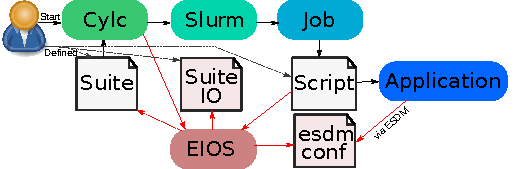
\includegraphics[scale=1.4]{stages-io}
  \caption{Software stack and stages of execution with our I/O-aware scheduler -- EIOS}
  \label{fig:stages-io}
\end{figure}


\begin{enumerate}

  \item \textbf{Cylc}
  Now, Cylc calls EIOS to identify potential optimisations in the schedule.
  EIOS may decide that subsequent jobs shall be placed on the same node or to reorder the execution of some jobs.
  Also, it may provide information for conducting data migration.

  \item \textbf{EIOS}
  The proposed system reads the information about the workflow (original and I/O suit files) and acts depending on the stage of the execution.
  EIOS consists of several subcomponents:
    \begin{itemize}
      \item The high-level scheduler that interfaces with Cylc.
      \item A tool that is run inside a script of a specific job/task -- as a replacement to the \texttt{cylc cycle-point} call.
      It generates pseudo file names that are used by the applications with ESDM support.
      \item A data management service (not shown on the figure) that purges or migrate data according to the user life cycle specification and the novelty information from EIOS.
    \end{itemize}
  EIOS components use the \texttt{esdm.conf} file that contains information about the available technology in the data centre and it provides the information on how to prioritise I/O targets.


  \item \textbf{Slurm}
  Cylc may now have added a constraint to place a job on the same node as a previous job and that is now handled by a modified Slurm.
  Also, if migrations have to be performed before or after a job, Slurm will administer them.

  \item \textbf{Job}
  A job might be scheduled on the same nodes than a previous job to utilize local storage.

  \item \textbf{Script}
  The way the filenames are generated is now different. A replacement command invokes EIOS to generate a pseudo filename.
  This filename will encode additional information for ESDM about how to prioritise data placement according to data access.
  Potentially, EIOS may generate an \texttt{esdm.conf} file for the specific application to adjust the mapping of data to available storage targets.

  \item \textbf{Application}
  The application may either use NetCDF with ESDM support or ESDM directly to access datasets.
  Hence, in \Cref{fig:layers}, the HDF5 layer is replaced with ESDM.
  ESDM loads the \texttt{esdm.conf} file that contains the information about the available storage backends and their configuration.
  ESDM extracts the long-term schedule information from the generated filenames and considers it during the I/O scheduling to exploit the data locality between tasks.

\end{enumerate}



\section{Conclusions}
\label{sec:conclusions}

Organising the data placement on storage tiers is typically performed manually by the developer/user or via policies, leading to suboptimal optimisations.
%On top of that, it is a tedious, non-portable, and error-prone task.
%Any hard-coded decision has significant implications for the performance of both applications and systems because the optimal choices about file size and content may be very different for the data production and any subsequent data analysis phase.
Manual and hard-coded workflows cannot handle changes in the environment and are error-prone.
Therefore, users must be able to express their workflows in an abstract fashion that allows the system to generate (near-)optimal execution plans and monitor their execution.

\section{Extra Figures}


\begin{figure}[H]
  \centering
  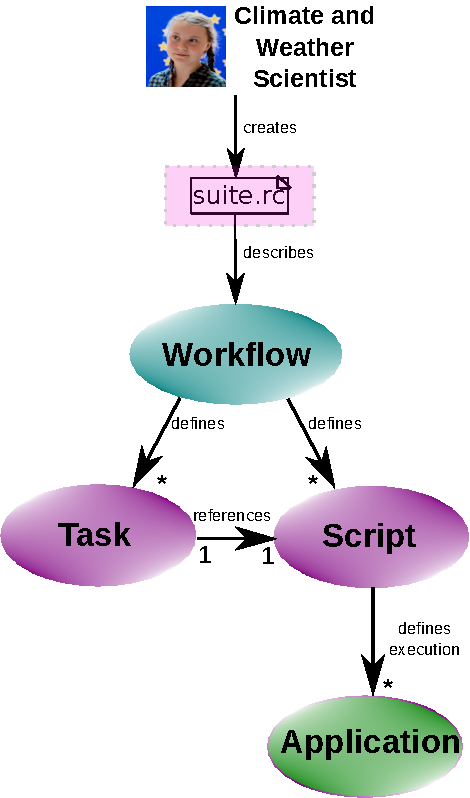
\includegraphics[scale=0.6]{workflow1-v2}
  \caption{Workflow 1.}
  \label{fig:work1}
\end{figure}

\begin{figure}[H]
  \centering
  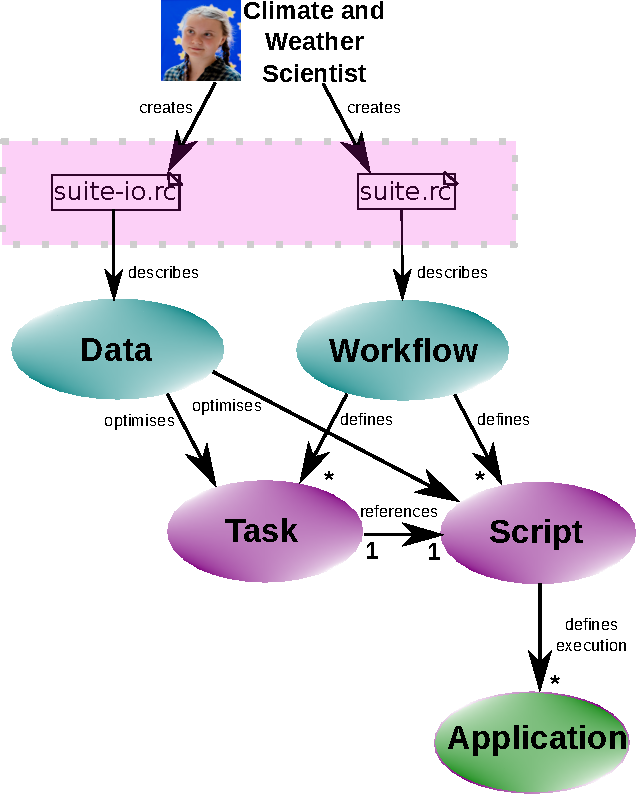
\includegraphics[scale=0.6]{workflow2-v2}
  \caption{Workflow 2.}
  \label{fig:work2}
\end{figure}

\begin{figure}[H]
  \centering
  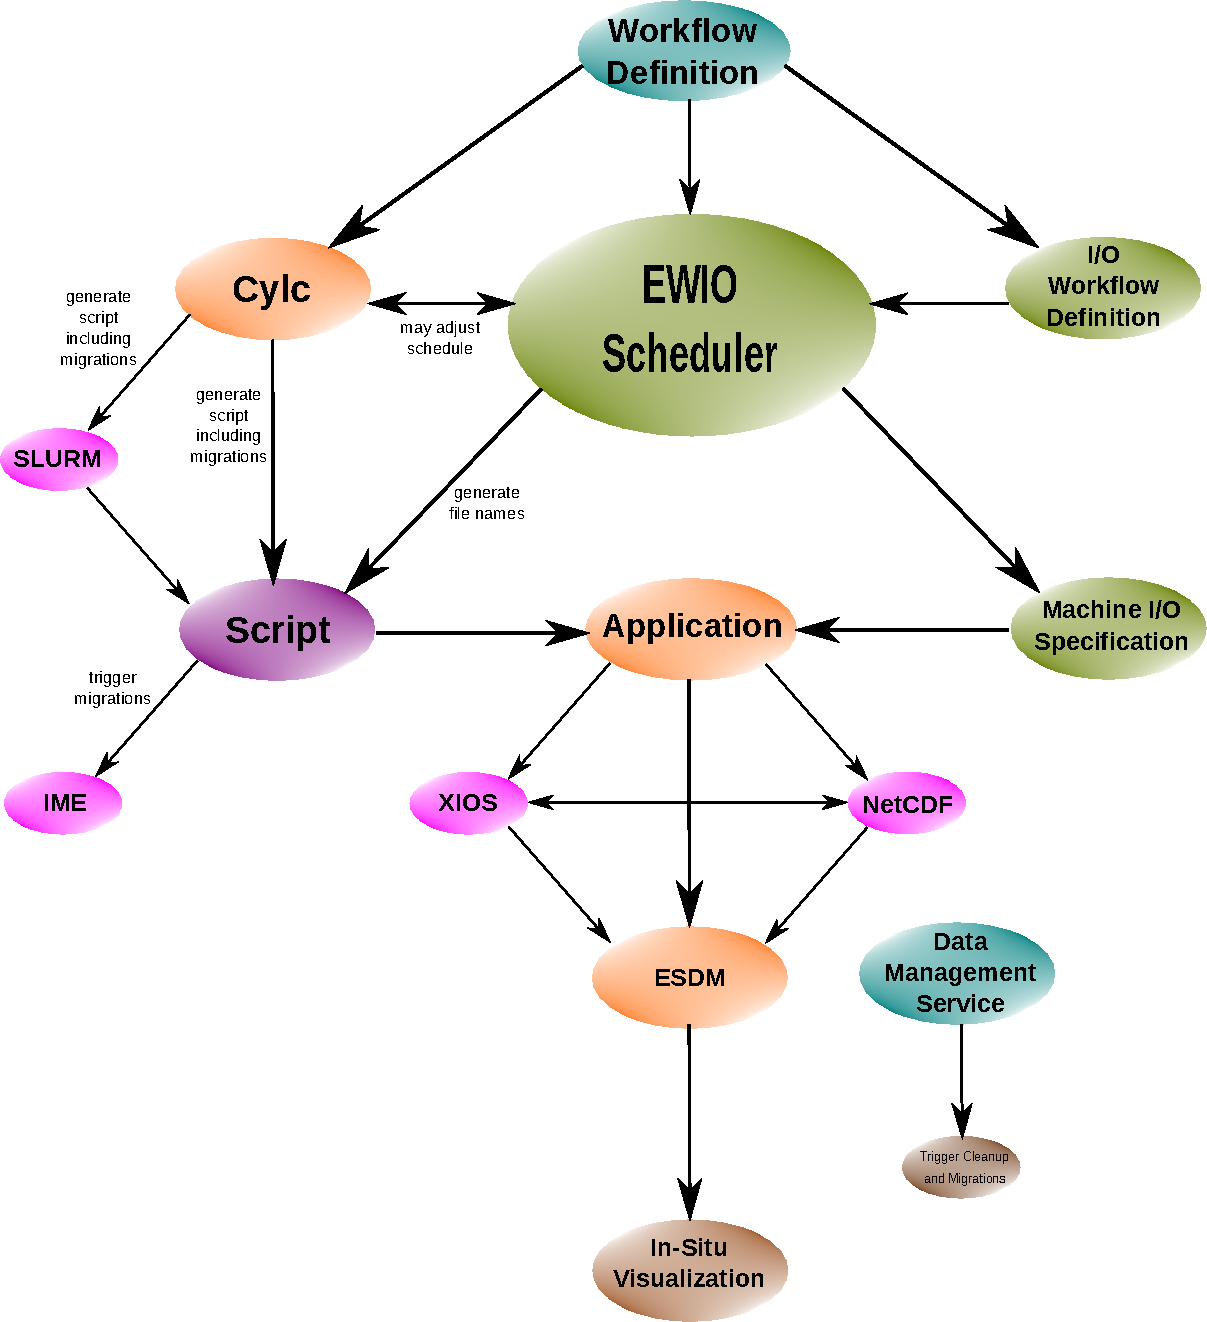
\includegraphics[scale=0.6]{workflow-all}
  \caption{Workflow All.}
  \label{fig:work}
\end{figure}

\begin{comment}

\begin{table}[H]
  \centering
  \begin{tabular}{cc}
  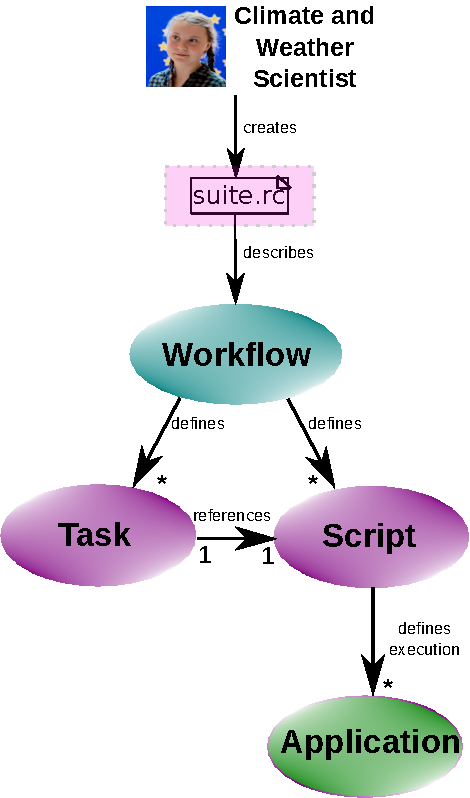
\includegraphics[scale=0.6]{workflow1-v2} &
  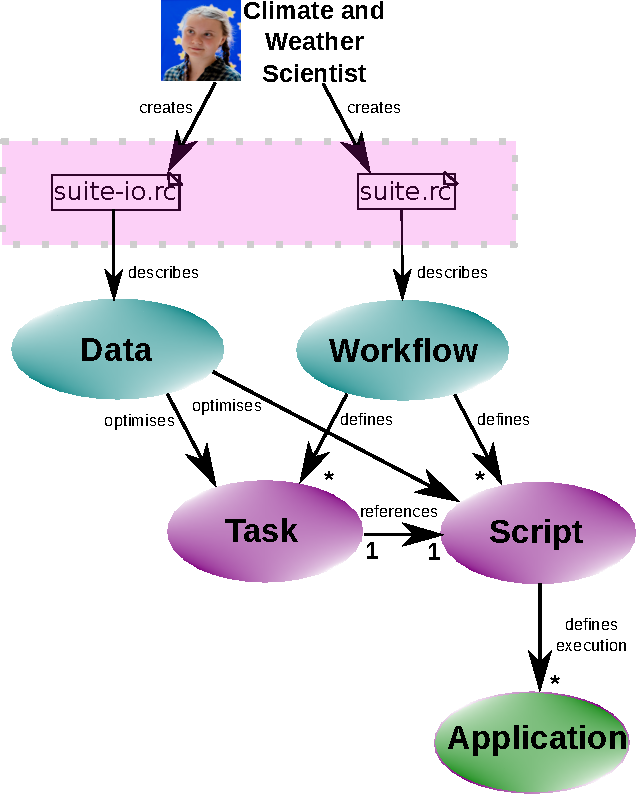
\includegraphics[scale=0.6]{workflow2-v2}
  \end{tabular}
  \caption{Workflows 1 and 2.}
  \label{fig:work1}
\end{table}

\end{comment}


\section{Specification of the Workflow from User Perspective}

From the user perspective, a general workflow can be described by three categories described in \Cref{tab:workflow}.

\begin{table}[H]
\centering
\begin{tabular}{|m{2cm}|m{5.5cm}|m{3.5cm}|m{3.5cm}|}
\hline
& \parbox{5.5cm}{\centering \textbf{Input}} & \parbox{3.5cm}{\centering \textbf{Computing}} & \parbox{3.5cm}{\centering \textbf{Products}} \\ \hline \hline

Description & information inserted in the workflow. & Tasks specified by the user. & Possible outcomes of the tasks. \\ \hline

\jk{?} File & \texttt{input.ds} & \texttt{tasks.ds} & \texttt{output.ds} \\ \hline

Composed of & Datasets/Scripts & Datasets/Scripts & Datasets \\ \hline

Information &

\begin{tabular}{m{5cm}}
\textbullet\ Dates for the experiments, how many times the workflow has to run, etc.\\
\textbullet\ Dependencies among the tasks.\\
\textbullet\ Information about the lifetime of the final outcome.\\
\textbullet\ Steps in which manual decisions have to be made.\\
\textbullet\ {{\color{cyan}{I/O information. (Where the datasets will be stored in each step of the workflow.)}}}\\
\end{tabular}

&

\begin{tabular}{m{3cm}}
\textbullet\ The data input.\\ \\
\textbullet\ The data output.\\ \\
\textbullet\ The data lifetime.\\ \\
\textbullet\ The dependencies regarding the other tasks.\\ \\
\textbullet\ {{\color{cyan}{I/O information.}}}
\end{tabular}

&

\begin{tabular}{m{3cm}}
\textbullet\ Datasets that will be used by other tasks.\\ \\
\textbullet\ Datasets that will generate the final output.\\
\end{tabular}

\\ \hline
\end{tabular}
\caption{Components of the workflow in the user perspective}
\label{tab:workflow}
\end{table}

For this work, Cylc is an essential tool regarding not only the execution of the workflow but the exchange of information with the EIOS about I/O and storage.
Cylc receives, as predefined, information about the storage and dependencies of the datasets. The current information is used to construct and run the complete workflow, but it is not employed in optimising intermediate steps.
The configuration is already predefined, and it cannot change. For instance, if it is established that Task\,2 depends on Task\,1, then we have to wait for Task\,1 to be completed to start running Task\,2.
Thinking what about I/O, no decision is being made about an optimal way to store the data.
Consider, as an example, that the datasets from \texttt{product1.ds} (the final product of task 1) are divided into \texttt{product1-final.ds} and \texttt{product1-task2.ds}. Then, it is clear that \texttt{product1-task2.ds} will be required to run Task\,2, and, because of that, should be put in fast storage to quickly being retrieved, or even kept in local storage. The \texttt{product1-final.ds} dataset, however, can go directly to tape, if the lifetime of the final output has to be stored for a long time, but no access is required from the current workflow.
The bottom line here is: several options can be optimised if we know the whole workflow in advance.


\begin{comment}

and computer-aided Research Development and Engineering (RD\&E)


and also on small-scale systems.

For example, Big data tools integrate computing and storage capabilities into a holistic solution demonstrating the benefit of tight integrating for data-driven workflows.

%-- the quality of service features available in hardware is rarely used.

Cloud definition of desired state and contracts.

Indeed many research prototypes address subproblems
* But not all aspects together
* Competing approaches; the standardisation we describe here does not compete!

In this paper, we purposely do not mention too many of the ongoing RD\&E in storage and computing.

To wrap up, NGI provides a high-level view on data and processing on heterogeneous platforms while shielding the user from execution details.

Open ...

%Kubernetes

\begin{description}

\item{NFS} Relatively slow, persistent file system - Nightly incremental backups

\item{Lustre} Large, fast distributed scratch file system - No backups

\url{https://info.hpc.sussex.ac.uk/hpc-guide/storage.html}

\end{description}

%, and data products are generated, which are processes that are executed outside of the first simulation.

\end{comment}

\bibliographystyle{alpha}
\bibliography{paper}

\end{document}
